{\chapter{PPO}}
\label{sec:ppo}
Das Unity ML-Agents Packet beinhaltet zwei bereits implementierte Algorithmen, SAC (Soft Actor Critic) und PPO (Proximal Policy Optimization). Beim testen der Walker Demo mit den zwei Algorithmen waren die Endergebnisse vergleichbar.
Jedoch hat der SAC Algorithmus in dieser Umgebung mehr Zeit gebraucht und das Lernverhalten war instabiler. Daher wird in der Arbeit der PPO Algorithmus von Open Ai verwendet. In diesem Kapitel wird die Funktionsweise hinter dem Algorithmus näher erklärt.

Der PPO Algorithmus basiert auf dem Akteur Kritik (Actor Critic) Ansatz. Der Akteur Kritik Ansatz nutz zwei neuronale Netze, das Akteur Netz lernt die Zuordnung von Zustand zu Aktion während das Kritik Netz bewertet wie gut es ist die Aktion zu wählen basierend auf dem aktuellen Zustand.

Akteur Verlust Funktion:
\begin{figure}[H]
  \centering  
  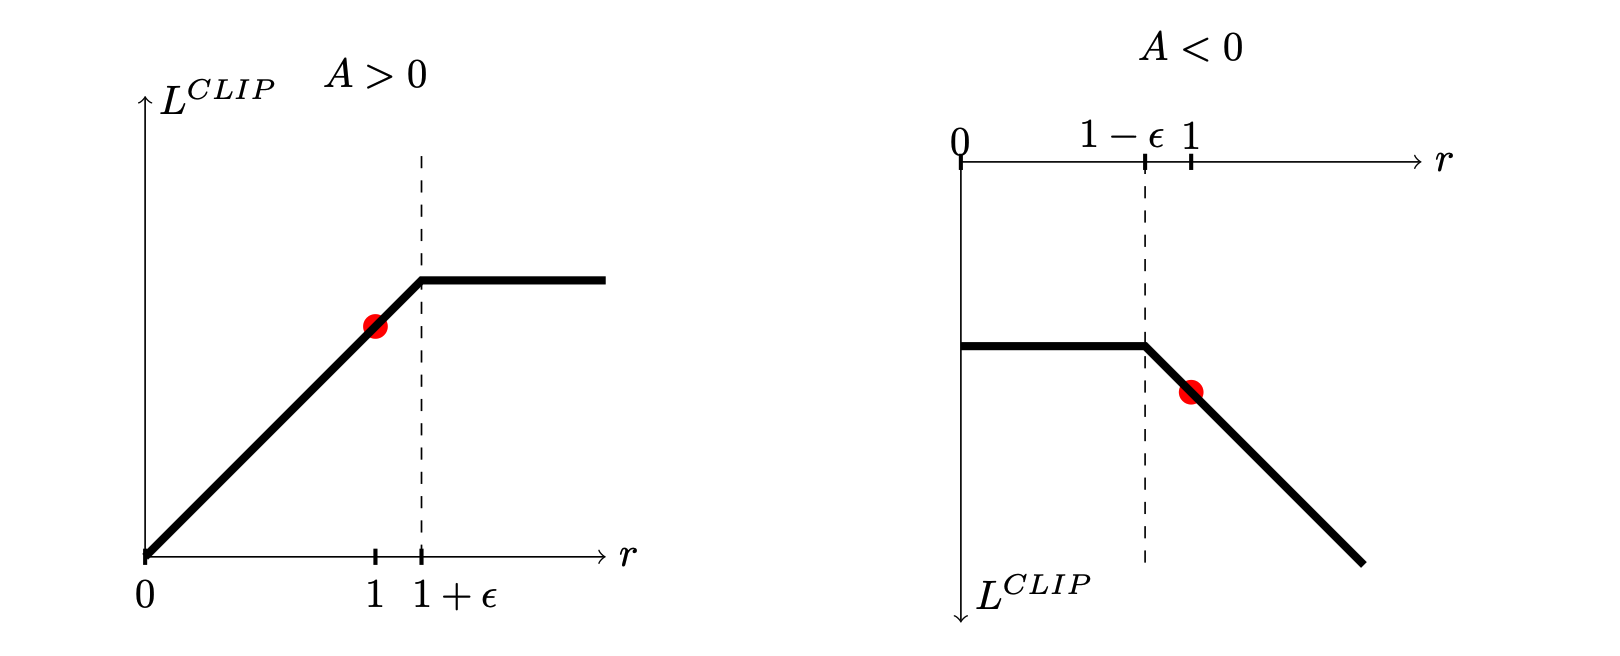
\includegraphics[scale=0.5]{img/ppo_clip.png}
  \caption{PPO Clip Funktion \protect\cite{schulman2017proximal}}
  \label{fig:ppo_clip}
\end{figure}

\begin{lstlisting}[caption={Codeausschnitt von Akteur Verlustfunktion aus Open Ai Spinning Up PPO implementation},captionpos=b]
ratio = torch.exp(logp - logp_old)
clip_adv = torch.clamp(ratio, 1-clip_ratio, 1+clip_ratio) * adv
loss_pi = -(torch.min(ratio * adv, clip_adv)).mean()
\end{lstlisting}

Kritik Verlust Funktion:
Um die Abweichung zwischen der Vorhersage des Kritik Netzes und dem tatsächlichen Ertrag zu messen nutzt PPO die mittlere quadratische Abweichung.
\begin{lstlisting}[caption={Codeausschnitt von Kritik Verlustfunktiion aus Open Ai Spinning Up PPO implementation},captionpos=b]
return ((ac.v(obs) - ret)**2).mean()
\end{lstlisting}